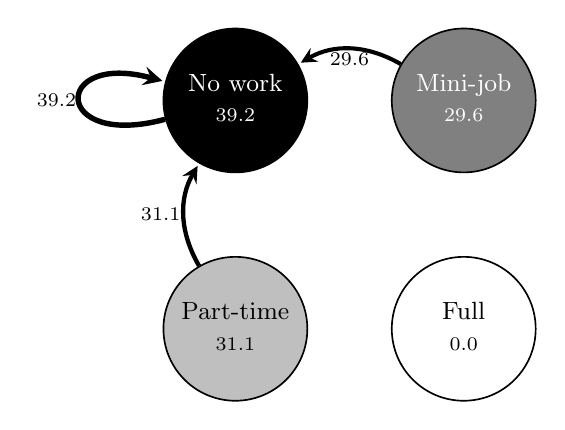
\begin{tikzpicture}[->,>=stealth,shorten >=1pt,auto,node distance=2.9cm, semithick] \tikzstyle{state}=[circle,fill=gray,draw=black,text=white]\node[state, fill=black,     minimum size=52pt, inner sep = -3pt]              (1)               {\small \begin{tabular}{c} No work  \\ {\scriptsize39.2}\end{tabular}}; \node[state, fill=gray,      minimum size=52pt, inner sep = -3pt]              (2) [right of=1]  {\small \begin{tabular}{c} Mini-job \\ {\scriptsize29.6}\end{tabular}}; \node[state, fill=lightgray, text=black, minimum size=52pt, inner sep = -3pt]  (3) [below of=1]  {\small \begin{tabular}{c} Part-time\\ {\scriptsize31.1}\end{tabular}}; \node[state, fill=white,     text=black,  minimum size=52pt, inner sep = -3pt] (4) [right of=3]  {\small \begin{tabular}{c} Full     \\ {\scriptsize0.0}\end{tabular}};\path(1) edge[line width=1.96pt,loop left,outer sep=-2pt] node {\scriptsize 39.2} (1)(2) edge[line width=1.48pt,bend right,outer sep=-2pt] node {\scriptsize 29.6} (1)(3) edge[line width=1.56pt,bend left,outer sep=-2pt] node {\scriptsize 31.1} (1); \end{tikzpicture} 